\section[Self-Induced Transparency \& Optical Solitons]
  {Self-Induced Transparency \& Optical Solitons\\ in Two-Level Atoms}
  \label{sec:sit}

  % \subsection{Introduction}  

    In chapter \ref{chp:propagation} we made first use of the Maxwell-Bloch
    propagation model to consider weak pulses of light incident on a medium of
    two-level atoms, and saw that it is possible to derive analytic solutions to
    these problems. Once we go beyond this linear regime, the approximations
    made in deriving those weak field solutions are not available, so in general
    the problem of nonlinear propagation must be solved numerically.

    There exists another set of conditions, however, that has proved susceptible
    to analytic description, and that is the case of short, strong pulses of
    light. By `short' here we specifically mean that the duration of the pulses
    is much shorter than the natural decay lifetime of the excited state, i.e.
    $\tau_w \ll \tau_\Gamma$. Strong, resonant interaction with light on this
    timescale results in a response from the atoms that is definitively 
    non-classical, as the interaction all happens within the phase memory of the
    atoms such that quantum-mechanical coherence is critical to understanding
    the propagation behaviour.

    Neglecting damping in this way, it must be the case that the total energy of
    the macroscopic atom-light system is a conserved quantity. We can express
    this conservation as
    \begin{equation}
      \left[ \frac{\partial}{\partial z} + 
      \frac{1}{c}\frac{\partial}{\partial t} \right]
      \lvert \mathcal{E} \rvert^2 + \frac{\partial U}{\partial t} = 0
    \end{equation}
    where $U$ is the matter energy density given by\cite{allen1975optical}
    \begin{equation}
      U = N \frac{\hbar \omega}{2} \int_{-\infty}^{\infty} \rho_{11} f(\Delta)  
      \dd \Delta.
    \end{equation}
    We must also have conservation of probability in the density matrix,
    such that
    \begin{equation}
      \Tr{\left[ \rho \right]} = \rho_{00} + \rho_{11} = 1  
    \end{equation}
    and it is this conservation law that distinguishes the semiclassical
    propagation model from any classical theory, with saturation of excitation
    inherent in two-level atoms that can story energy only of $\hbar \omega_0$.
    The phenomena of self-induced transparency (\textsc{sit}) we shall discuss
    in this section is one interesting result of such saturation effects.

  \subsection{The Area Theorem}  

    A central tool for describing the propagation of short, strong pulses is the
    nonlinear \textit{area theorem}.\cite{McCall1969} The concept of the pulse
    area generalises the Rabi frequency from steady fields such that it is
    useful for the description of time-dependent field envelopes. We define the
    pulse area by
    \begin{equation}
      \theta(z) = \int^{\infty}_{-\infty} \Omega(z, \tau) \dd \tau
      \label{eqn:pulse_area}
    \end{equation}
    where $\Omega(z, \tau)$ as before is the Rabi frequency envelope of the
    pulse.

    Inserting this definition for $\theta(z)$ into the expression we derived for
    the time-evolution of the electric field envelope ([REF]) and taking the
    analytic expression for Rabi oscillation of the atomic coherence $\rho_{01}$
    on resonance [REF], it is possible to derive an expression for the evolution
    of the pulse area as the pulse propagates through the medium
    \begin{equation}
      \frac{\partial}{\partial z} \theta(z) = -\frac{\alpha}{2} \sin{\theta(z)}
      \label{eqn:area_theorem}
    \end{equation}
    where $\alpha$ is the resonant absorption coefficient defined in equation
    (\ref{eqn:beer_law}). In the case of weak fields such that $\theta(z) \ll 1$
    we may approximate $\sin{\theta(z)} = \theta$ and obtain the Beer absorption
    law, which we thus see is generalised by the area theorem. [TODO FIX REFS]

  \subsection{Self-Induced Transparency} 

    Now looking at the case of a pulse of light with a time-dependent profile
    such that $\theta(z) = 2\pi$, we see that equation (\ref{eqn:area_theorem})
    tells us $\nicefrac{\partial \theta}{\partial z} = 0$, \ie that the area of
    the pulse will remain constant.

    This suggests that it is possible for some form of $2\pi$ pulse to travel
    through the medium without attenuation. This indeed turns out to be the case
    if the envelope profile is such that the Bloch vector is rotated along
    a specific trajectory, effected by a hyperbolic secant profile
    \begin{equation}
      \Omega_{2\pi}(z, \tau) = \frac{2}{\tau_{s}} 
          \sech\left(\frac{\tau - \nicefrac{z}{v_g}}{\tau_s}\right)
      \label{eqn:sech_shape}
    \end{equation}
    where $\tau_s$ defines the width of the pulse and $v_g$ is the group
    velocity.

    \begin{figure}[]
      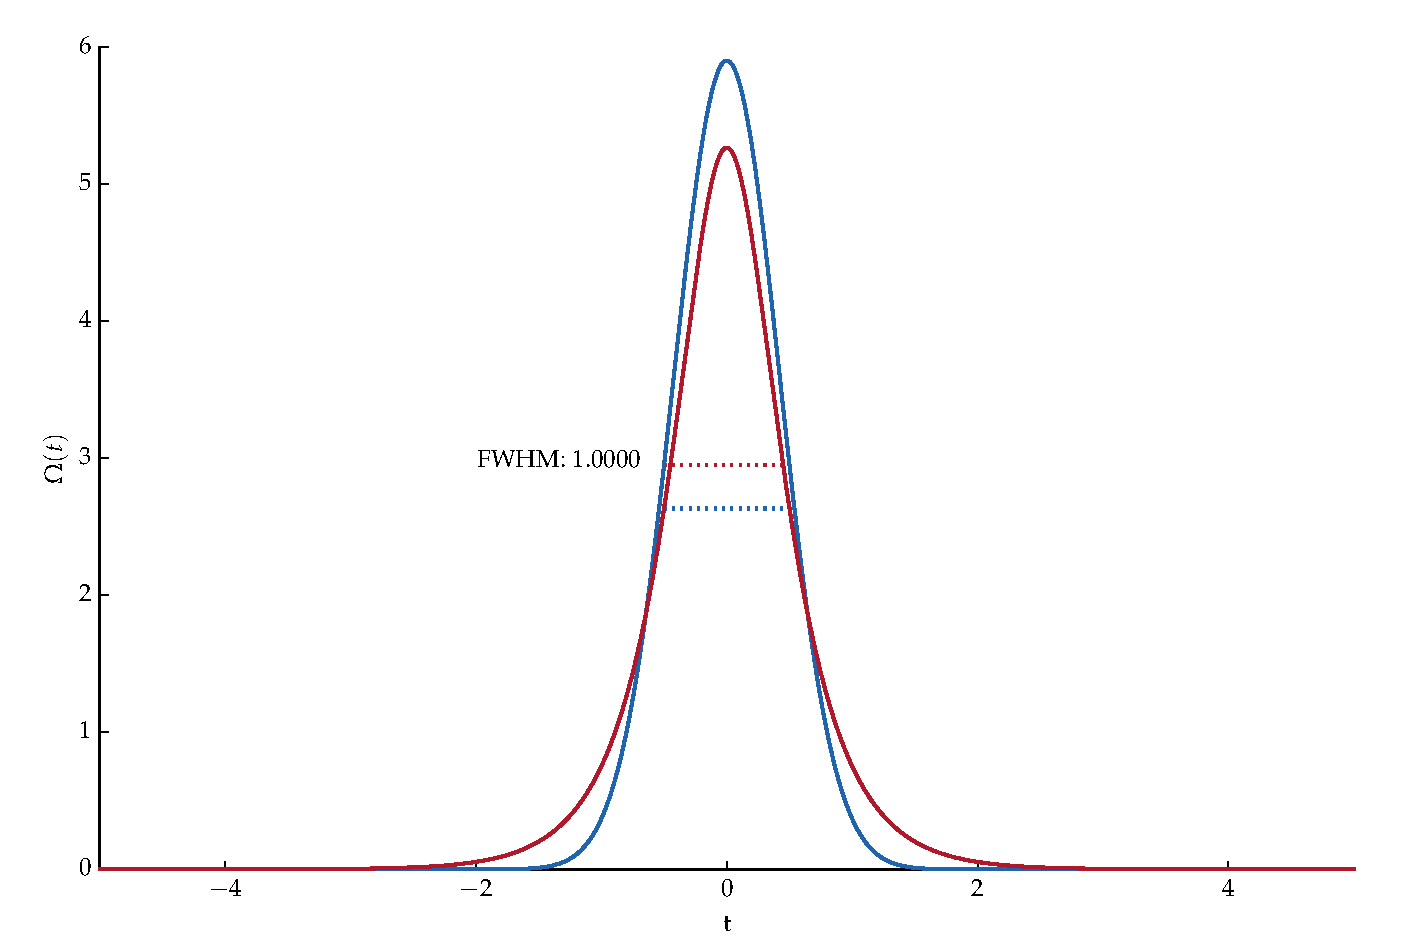
\includegraphics[width=\linewidth]
        {figs/03_nonlinear/plot_sech_vs_gaussian_fig1.pdf}
      \caption{
      The hyperbolic secant function (red) expressed in equation
      (\ref{eqn:sech_shape}) and Gaussian (blue) expressed in equation
      (\ref{eqn:gaussian}). Both have pulse area $\theta = 2\pi$ and
      \textsc{fwhm} $\tau_w = \unit[1.0]{}$. The \textsc{fwhm}s are indicated
      with dotted lines.
      }
      \label{fig:sech_vs_gaussian}
    \end{figure}

    In figure \ref{fig:sech_vs_gaussian} we show the hyperbolic secant function
    expressed in equation (\ref{eqn:sech_shape}) and compare it with the
    familiar Gaussian profile of equation (\ref{eqn:gaussian}) of the same pulse
    area $\theta = 2\pi$ and \textsc{fwhm} $\tau_w = \unit[1.0]{}$. We see that
    these functions are similar but that the sech function has a smaller peak
    amplitude and larger wings. We determine numerically that the \textsc{fwhm}
    is related to the sech-width $\tau_s$ via $\tau_s \approx $
    \unit[$2.633916$]{$\tau_w$}.
    
    The group velocity, relative to the speed-of-light reference frame, is given
    by
    \begin{equation}
      v_g = \frac{2}{Ng \cdot t_s^2}
      \label{eqn:soliton_group_velocity}
    \end{equation}
    which means that the exit of the envelope from the medium is delayed
    relative to an equal travel distance in vacuo by $L/v_g$.

    \begin{figure}[]
      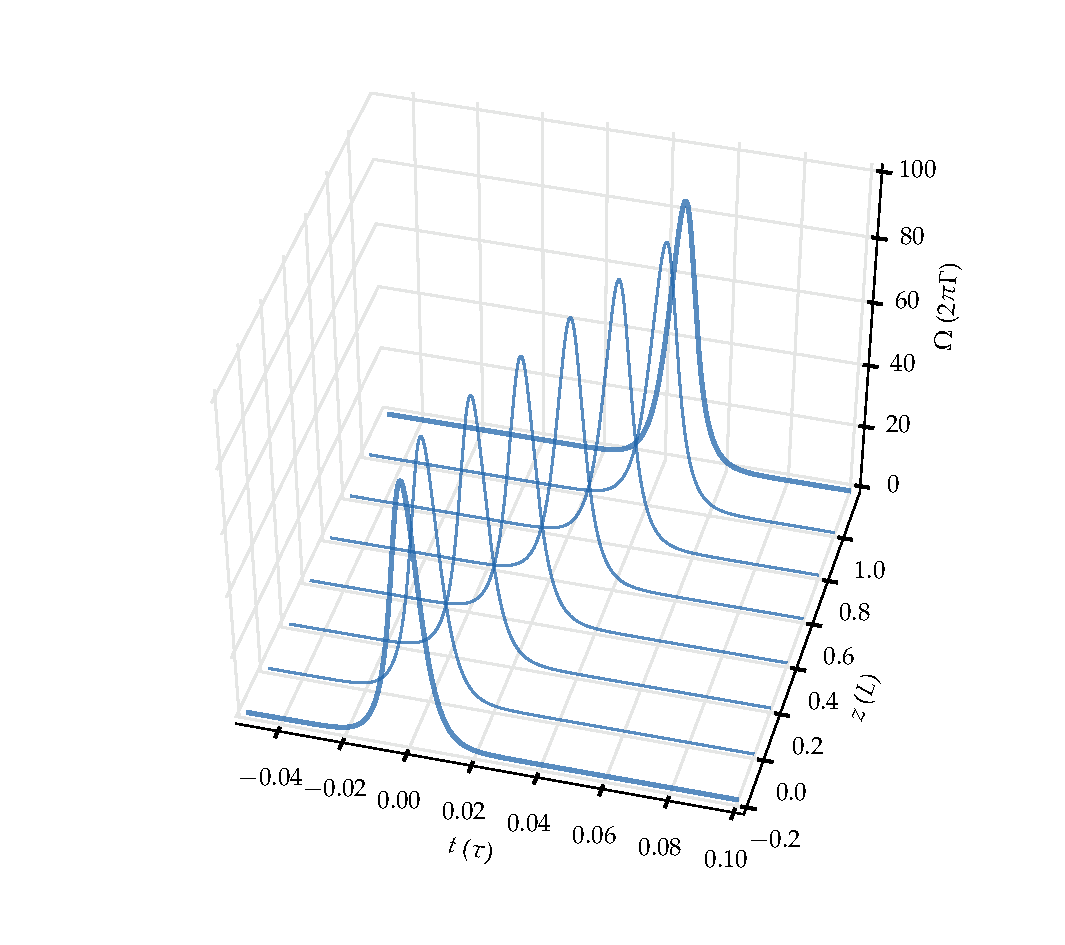
\includegraphics[width=\linewidth]
        {figs/03_nonlinear/coh_sech_2_0pi_fwhm0_010_Ng01000_fig4.pdf}
      \caption{
      Simulated absolute value of the complex Rabi frequency $\Omega(z, \tau)$
      for the propagation of a $\theta = 2\pi$ sech pulse of \textsc{fwhm}
      $\tau_w = $ \unit[0.01]{$\tau_\Gamma$} through a medium with
      constant density such that $Ng = \unit[2\pi~10^3]{\Gamma/L}$.
      }
      \label{fig:2pi_sech_simulton_3d}
    \end{figure}

    In figure \ref{fig:2pi_sech_simulton_3d} we show the results of a
    simulation, again using the numerical scheme defined in appendix
    \ref{apx:mb_eqns}, of the absolute part of the Rabi frequency $\Omega(z,
    \tau)$ for the propagation of a $\theta = 2\pi$ sech pulse through a medium
    of two-level atoms. The pulse has a \textsc{fwhm} $\tau_w = $
    \unit[0.01]{$\tau_\Gamma$} and the medium is defined such that $Ng =
    \unit[2\pi~10^3]{\Gamma/L}$.

    We see that the $2\pi$ pulse retains its profile through the medium, but is
    delayed by \unit[$\approx 0.05$]{$\tau_\Gamma$}. Recall that in the
    speed-of-light reference frame shown in these figures, a pulse of light in
    vacuo arrives at the same time it left.

    \begin{figure}[]
      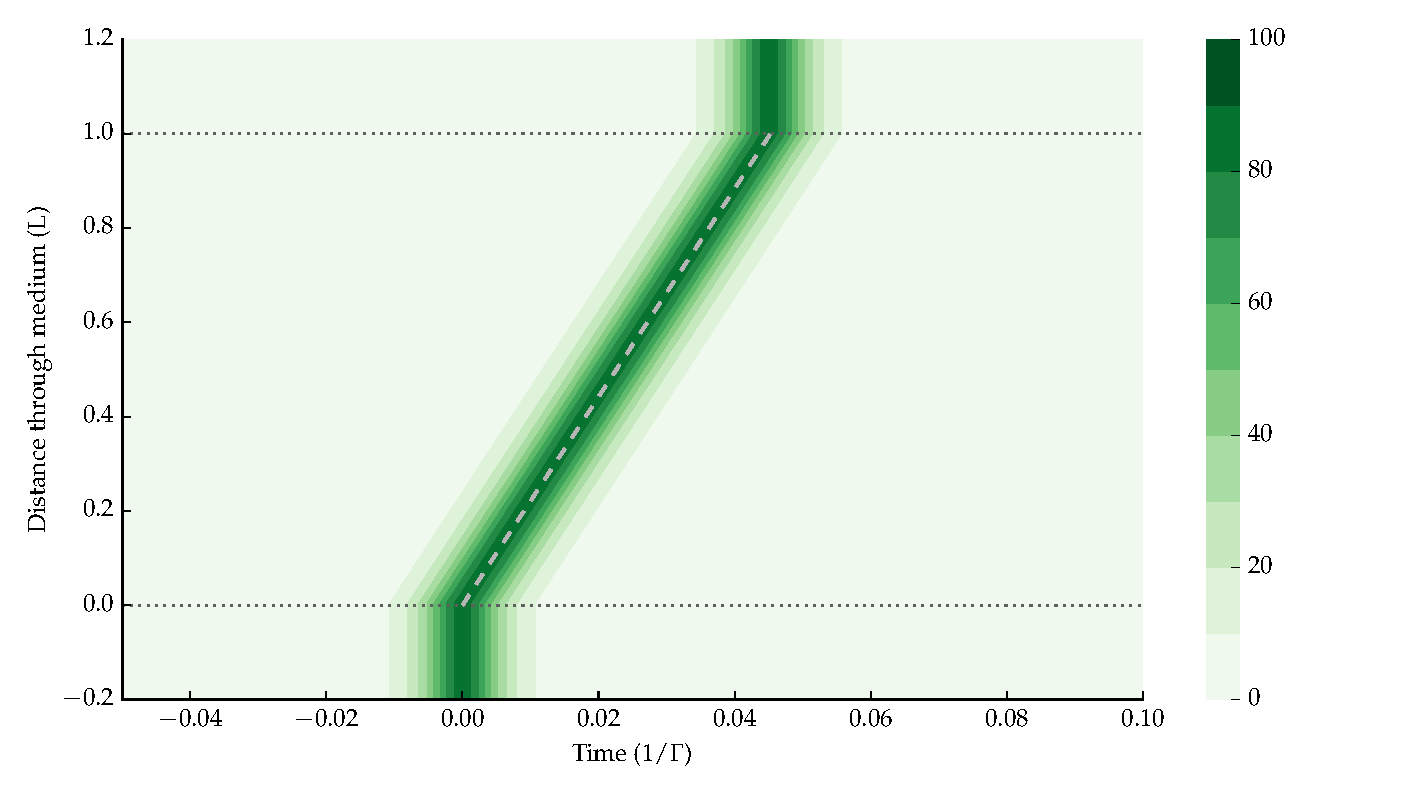
\includegraphics[width=\linewidth]
        {figs/03_nonlinear/coh_sech_2_0pi_fwhm0_010_Ng01000_fig1.pdf}
      \caption{
      Colormap showing the same simulated results shown in figure
      \ref{fig:2pi_sech_simulton_3d}. The dotted lines at $z = \unit[0, 1]{L}$
      mark the start and end of the medium. The dashed line indicates the
      analytic pulse velocity given in equation
      (\ref{eqn:soliton_group_velocity}).
      }
      \label{fig:2pi_sech_simulton}
    \end{figure}

    In figure \ref{fig:2pi_sech_simulton} we show the same result as a colour
    map, from which we can more clearly see both the consistency of the pulse
    profile as it propagates through the medium and the slower group velocity.
    The analytic pulse velocity, given in equation
    (\ref{eqn:soliton_group_velocity}), is shown by the dotted line, and we see
    that the pulse peak matches that result.

    \begin{figure}[]
      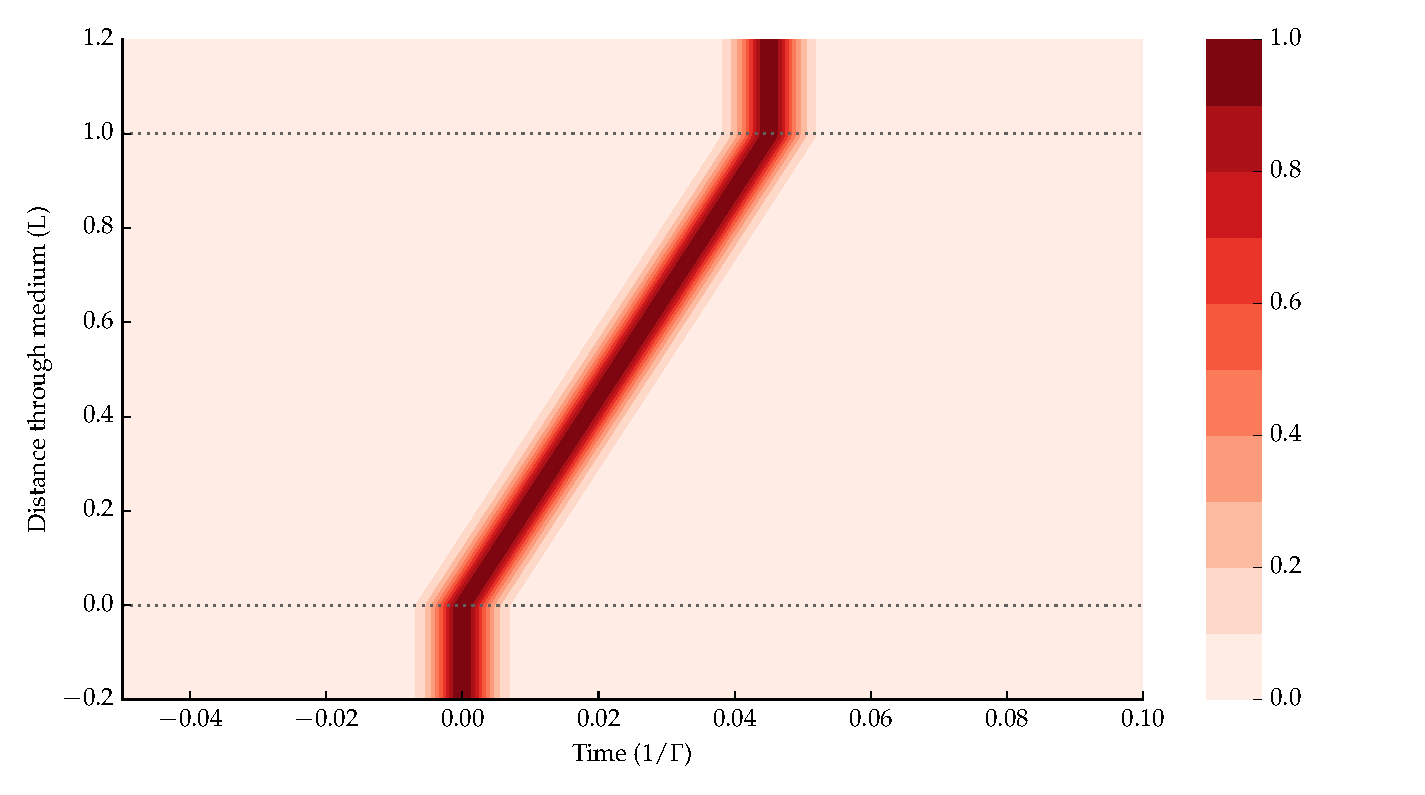
\includegraphics[width=\linewidth]
        {figs/03_nonlinear/coh_sech_2_0pi_fwhm0_010_Ng01000_fig2.pdf}
      \caption{
        Simluated excited state population $\rho_{11}$ for the propagation of a
        $\theta = 2\pi$ sech pulse of \textsc{fwhm} $\tau_w = $
        \unit[0.01]{$\tau_\Gamma$} through a medium with constant density such
        that $Ng = \unit[2\pi~10^3]{\Gamma/L}$.
      }
      \label{fig:2pi_sech_simulton_pop}
    \end{figure}

    \begin{figure}[]
      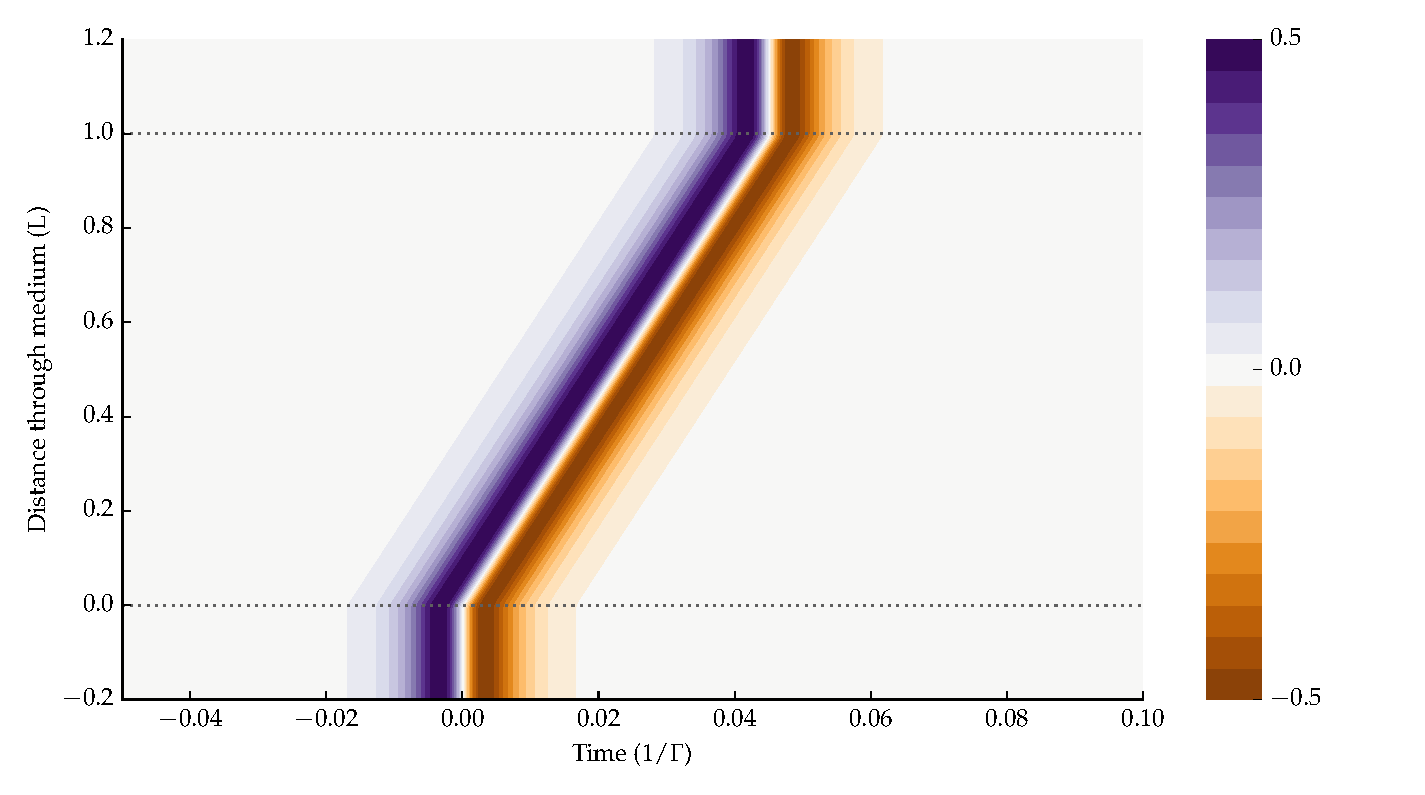
\includegraphics[width=\linewidth]
        {figs/03_nonlinear/coh_sech_2_0pi_fwhm0_010_Ng01000_fig3.pdf}
      \caption{
        Simluated imaginary coherence $\Im{\rho_{01}}$ for the propagation of a
        $\theta = 2\pi$ sech pulse of \textsc{fwhm} $\tau_w = $
        \unit[0.01]{$\tau_\Gamma$} through a medium with constant
        density such that $Ng = \unit[2\pi~10^3]{\Gamma/L}$.
      }
      \label{fig:2pi_sech_simulton_coh}
    \end{figure}

    We can understand the reason the pulse is able to travel without attenuation
    by looking at elements of the density matrix. 

    Figure \ref{fig:2pi_sech_simulton_pop} shows the excited state population
    $\rho_{11}$. We see that at each point in space through the medium, the
    pulse transfers all of the population to the excited state as the atoms
    absorb energy from the field, before returning it completely to the ground
    state.

    In figure \ref{fig:2pi_sech_simulton_coh} we consider the imaginary part of
    the coherence $\Im\left[{\rho_{01}}\right]$. We see that at each point in space through
    the medium, this makes a complete oscillation.

    Note that due to the form of the simulation, the results show atomic
    populations outside of the area of the medium area. We may consider the
    number density $N$ to be arbitrarily close to zero in these regions.

    As the sech pulse moves through the medium, its leading edge inverts each
    slice of the atomic population via absorption before its trailing edge
    returns the population to the ground state by stimulated
    emission.\cite{Lamb1971} The fact that we are in the regime where we may
    neglect spontaneous decay means that this rotation happens entirely within
    the phase memory of the atoms, and no energy is taken from the pulse. This
    phenomenon is known as \textit{self-induced transparency} (\textsc{sit}) as
    it is the area of the pulse itself which makes the medium transparent to it,
    and is an example of an optical soliton\cite{kivshar2003optical}.

    We can understand that the group velocity $v_g$ must necessarily be less
    than $c$ due to the fact that the pulse energy spends some non-zero amount
    of its time as an excitation in the non-moving medium.

    \begin{figure}[]
      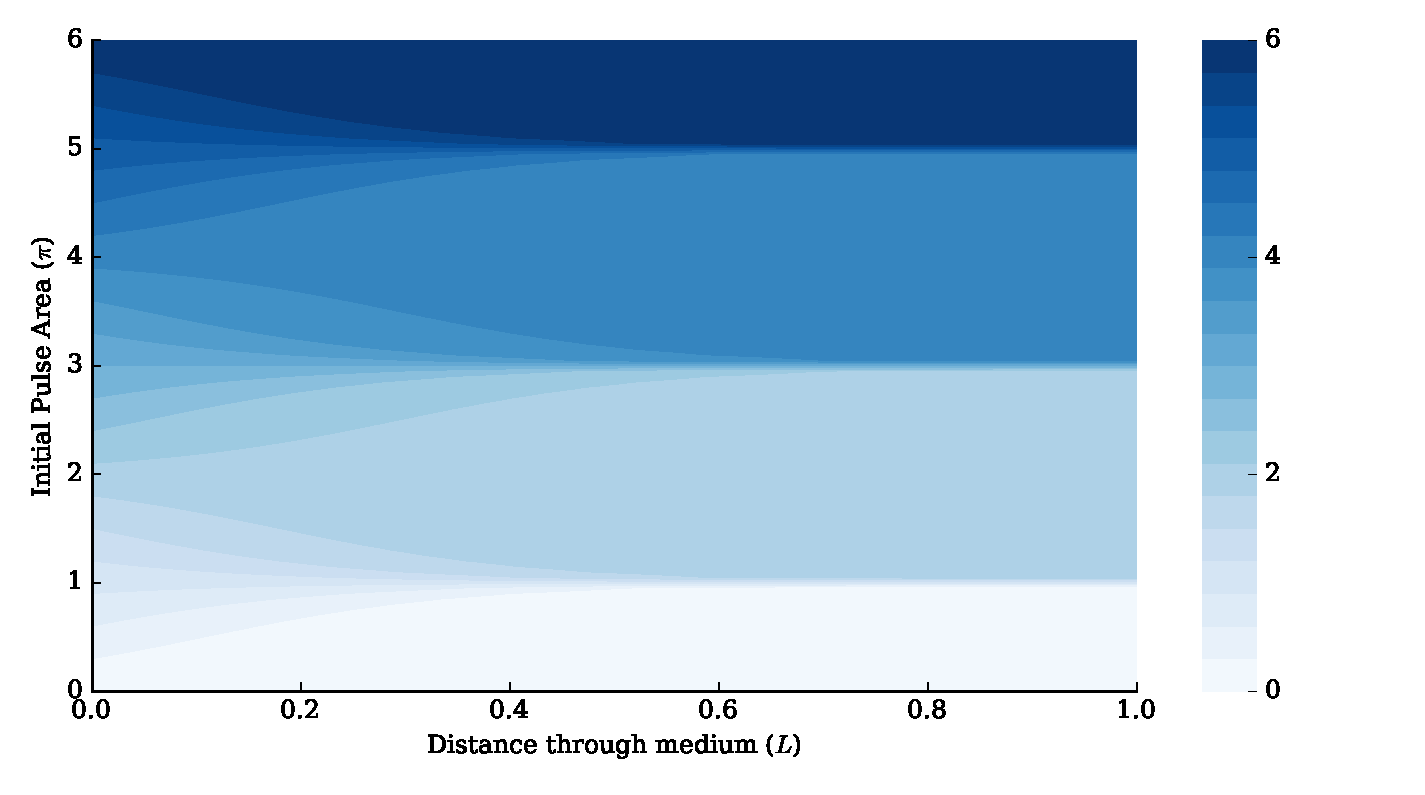
\includegraphics[width=\linewidth]
        {figs/03_nonlinear/plot_area_theorem_cmap_fig1.pdf}
      \caption{
        The pulse area $\theta(z)$ solution to the area theorem differential
        equation (\ref{eqn:area_theorem}) as a function of distance $z$ and
        initial pulse area $\theta_0(z)$ from $0$ to $6\pi$ for an absorption
        coefficient $\alpha =  \unit[2\pi~2]{\Gamma/L}$.
      }
      \label{fig:area_theorem_cmap}
    \end{figure}

    We are next led to consider the effect of applying a pulse of an area that
    is not exactly $2\pi$ or of a different shape to the sech profile. In figure
    \ref{fig:area_theorem_cmap} we show the result of integration of the area
    theorem differential equations over a range of input pulse areas,
    representing the initial condition, from $0$ to $6\pi$ for an absorption
    coefficient $\alpha =  \unit[2\pi~2]{\Gamma/L}$. We observe that these
    inputs converge on stable solutions at the nearest even multiple of $\pi$
    (i.e. $\theta(z) \rightarrow 0$, $2\pi$, $4\pi$, $\dots$).

    \begin{figure}[]
      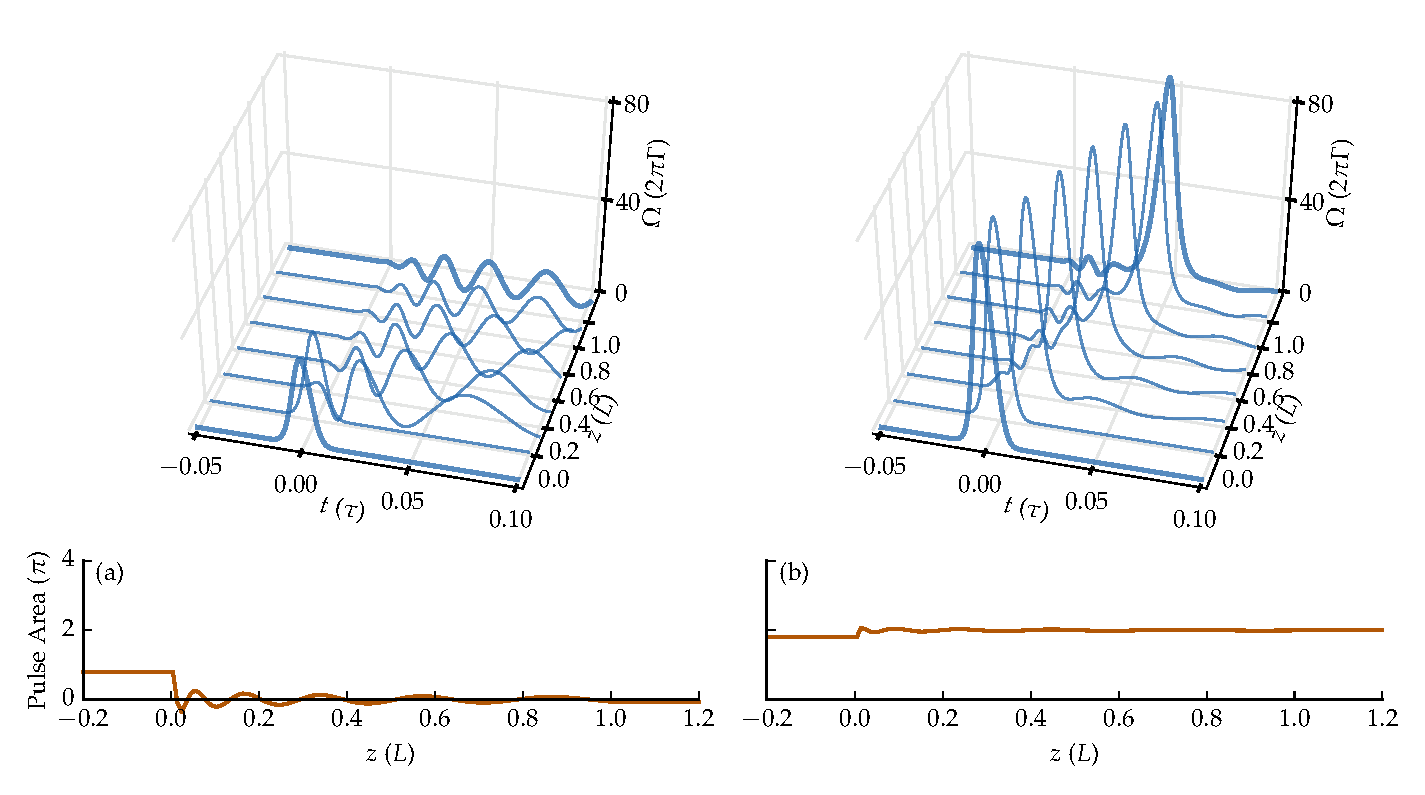
\includegraphics[width=\linewidth]
        {figs/03_nonlinear/coh_gaus_plot_0_8pi_1_8pi_fwhm0_010_N01000_fig1.pdf}
      \caption{
      Propagation of (a) $0.8 \pi$ and (b) $1.8 \pi$ pulses, showing (top)
      profiles of the real part of the complex Rabi frequency $\Omega(z, \tau)$
      and (bottom) pulse area $\theta(z)$.
      }
      \label{fig:sit_08_18_nodecay}
    \end{figure}

    In figure \label{fig:ref} we demonstrate the effect of \textsc{sit} for the
    propagation of resonant input pulses of $0.8 \pi$ and $1.8 \pi$
    respectively. Both input pulses are Gaussians of width $\tau_w = $
    \unit[0.01]{$\tau_\Gamma$} and the medium is such that $Ng_{01} =
    \unit[2\pi~10^3]{\Gamma/L}$.

    We see that for the $0.8 \pi$ pulse in figure \ref{fig:sit_08_18_nodecay}
    (a) the area $\theta(z)$ rapidly attenuates soon after entering the medium.
    The pulse energy is not entirely absorbed, however. The pulse bandwidth is
    much wider than the absorption window but still prone to dispersion and so
    the envelope is distorted and we see high-frequency ringing through the
    medium.

    In clear contrast, for the $1.8 \pi$ pulse in figure
    \ref{fig:sit_08_18_nodecay} (b) the area $\theta(z)$ tends to $2\pi$ and the
    profile steepens and narrows into the sech-type soliton which propagates
    without absorption. We thus observe that the input pulse \textit{does not
    need} to be of the sech profile to be capable of propagating as an optical
    soliton as the medium can shape the pulse into that profile as it propagates
    if the pulse area $\theta(z) > \pi$.

    We note again that the group velocity $v_g$ is lower than $c$ due to the
    energy of the field spending some amount of its time as an excitation in the
    fixed medium.

  \subsection{Pulse Breakup} 

    For pulses $>3 \pi$, the area theorem predicts that the area will tend to
    the the nearest even multiple of $\pi$, but in fact there are no steadystate
    solutions to the propagation problem other than the $2\pi$ sech
    pulse\cite{Matulic1972}. In larger pulses, we find that the Rabi frequency
    envelope breaks into discrete $2\pi$ envelopes with different widths and
    thus group velocities\cite{Lamb1971}.

    \begin{figure}[]
      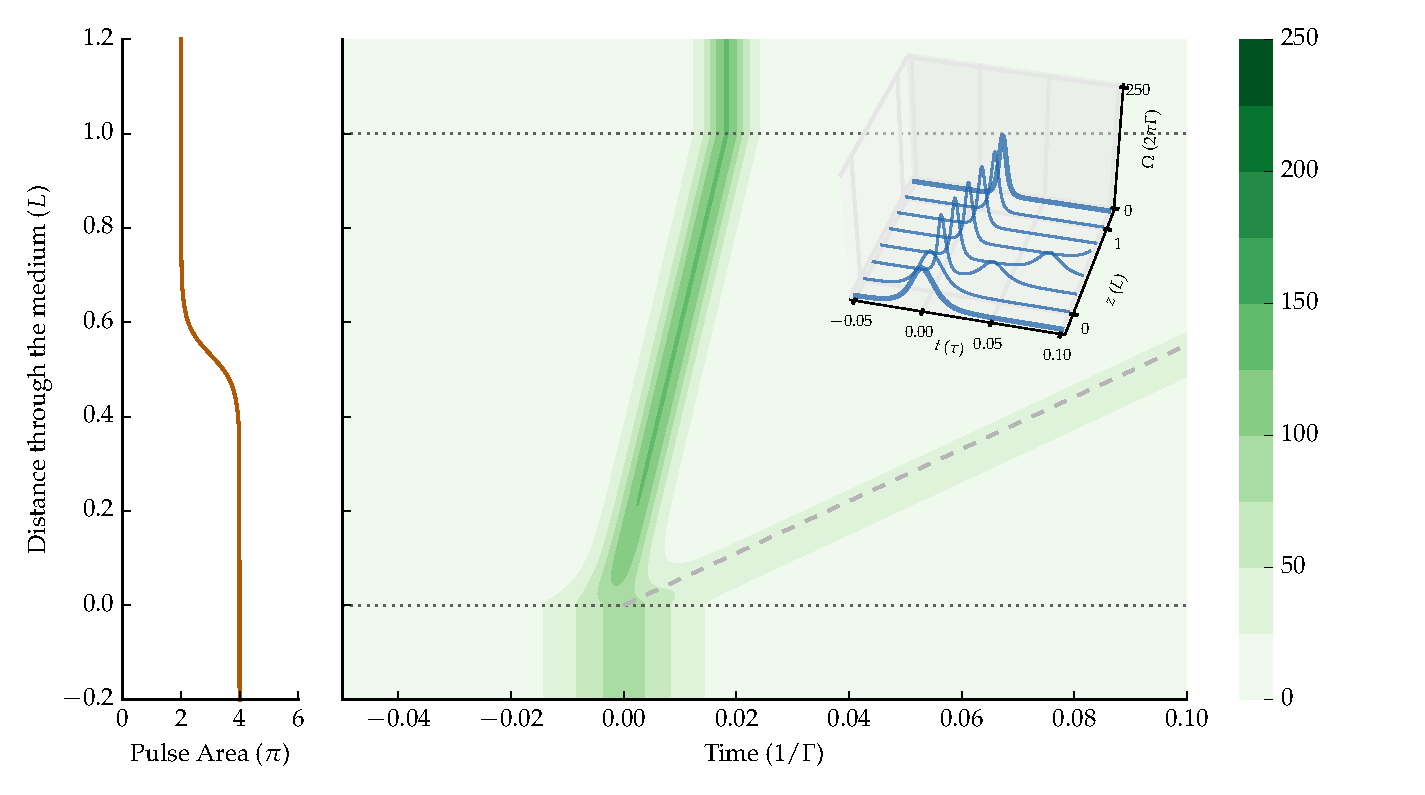
\includegraphics[width=\linewidth]
        {figs/03_nonlinear/coh_sech_4_0pi_fwhm0_020_Ng01000_fig5.pdf}
      \caption{
      Propagation of a $4 \pi$ sech-type pulse. (main colourmap) Absolute value
      of the complex Rabi frequency $\Omega(z, \tau)$. The dashed line indicates
      the analytic pulse velocity given in equation
      (\ref{eqn:soliton_group_velocity}). (inset \textsc{3d}) Propagation
      profile of the pulse. (left) pulse area $\theta(z)$.
      }
      \label{fig:sit_4pi}
    \end{figure}

    \begin{figure}[]
      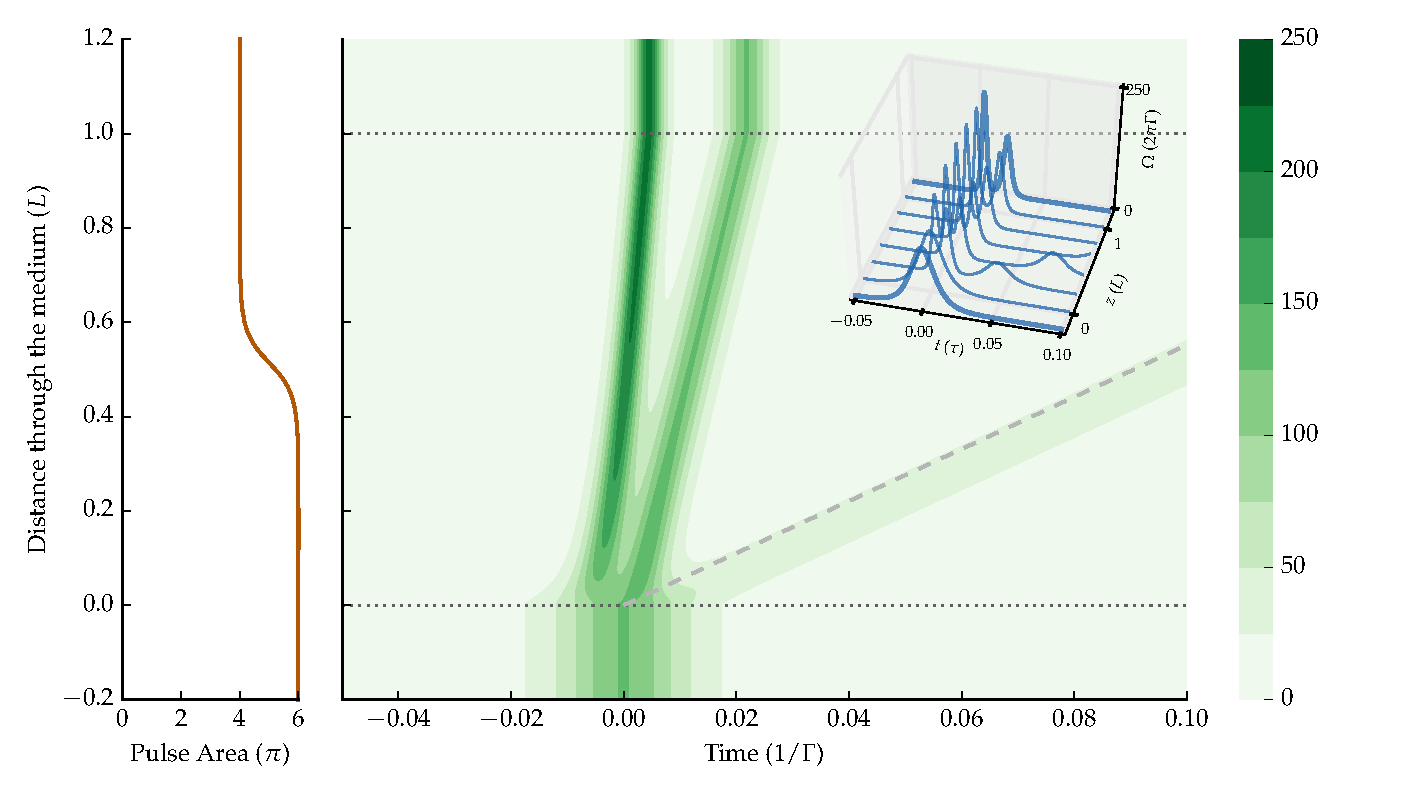
\includegraphics[width=\linewidth]
        {figs/03_nonlinear/coh_sech_6_0pi_fwhm0_020_Ng01000_fig6.pdf}
      \caption{
      Propagation of a $6 \pi$ sech-type pulse. (main colourmap) Absolute value
      of the complex Rabi frequency $\Omega(z, \tau)$. (inset \textsc{3d})
      Propagation profile of the pulse. (left) pulse area $\theta(z)$.
      }
      \label{fig:sit_6pi}
    \end{figure}

    In figures \ref{fig:sit_4pi} and \ref{fig:sit_6pi} we see the result of
    $4\pi$ and $6\pi$ sech-type pulses of width $\tau_w =$
    \unit[0.02]{$\tau_\Gamma$} through a medium with $Ng =
    \unit[2\pi~10^3]{\Gamma/L}$. Again we neglect the spontaneous decay of the
    excited state. We see that the pulse immediately breaks up on entering the
    medium and that the resultant pulses steepen into sech-type solitons just
    like the single $2\pi$ pulse.    

    The resultant pulses have different widths and thus different group
    velocities as predicted in equation (\ref{eqn:sech_shape}), though we see
    that the final resultant pulse travels at the same velocity as an incident
    $2\pi$ pulse of the same original width. The area subplots confirm that the pulse area of each resultant pulse is the steady-state solution, $2\pi$.

    \begin{figure}[]
      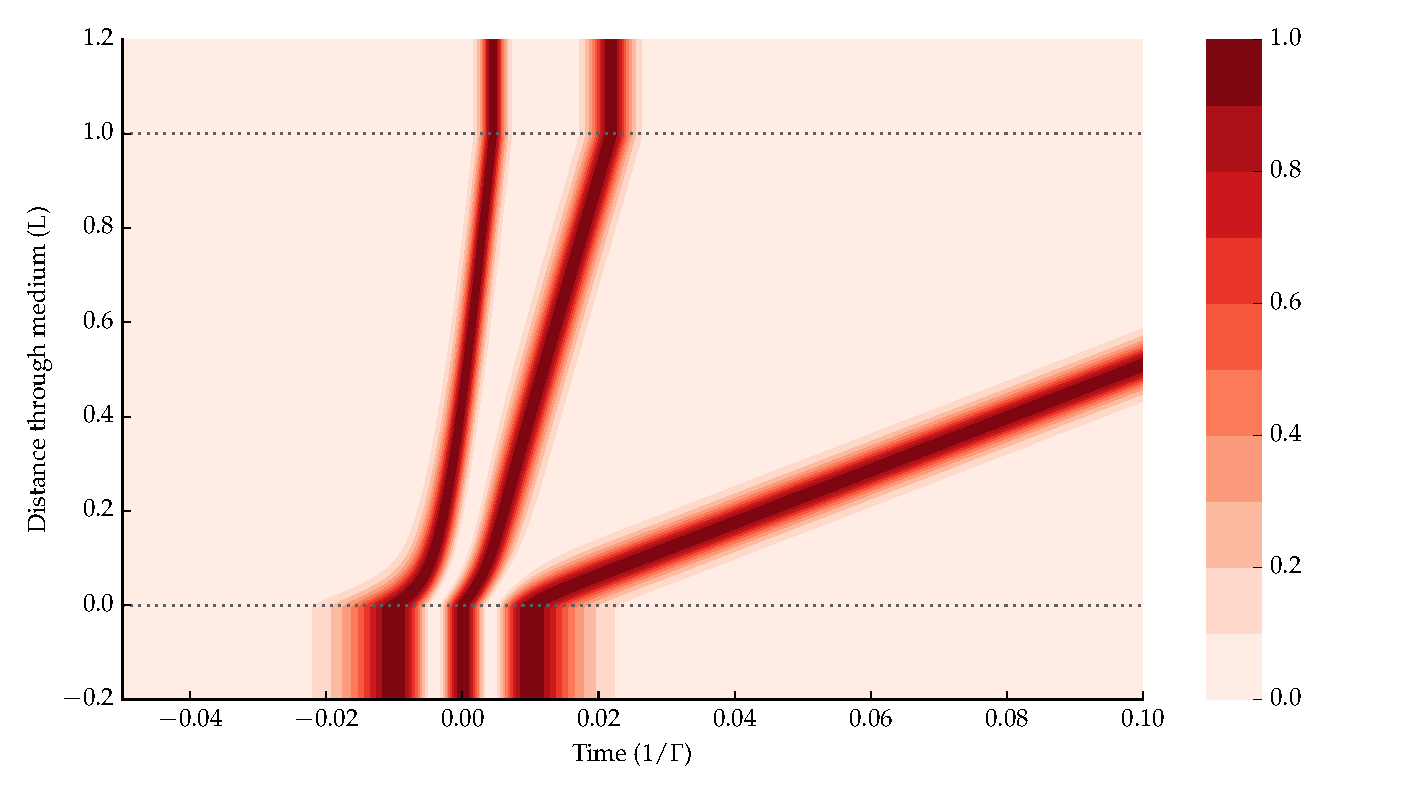
\includegraphics[width=\linewidth]
        {figs/03_nonlinear/coh_sech_6_0pi_fwhm0_020_Ng01000_fig3.pdf}
      \caption{
        Simluated excited state population $\rho_{11}$ for the propagation of a
        $\theta = 6\pi$ sech pulse of \textsc{fwhm} $\tau_w = $
        \unit[0.02]{$\tau_\Gamma$} through a medium with constant density such
        that $Ng = \unit[2\pi~10^3]{\Gamma/L}$.
      }
      \label{fig:sit_6pi_pop}
    \end{figure}

    Figure \ref{fig:sit_6pi_pop} shows the excited state population $\rho_{11}$
    corresponding to the $6\pi$ sech pulse. We see that the resultant pulses
    emerge from each of the three full Rabi oscillations made by the $6\pi$
    pulse.

    The first paper by McCall and Hahn describing \textsc{sit} theoretically
    included experimental evidence of the effect.\cite{McCall1969} Results were
    presented from an experiment using a liquid-helium ruby absorber showing
    that intense light transmitted without attenuation but delayed. In such
    early experiments however it was difficult to discount the possibilty of a
    hole-burning effect, where the absorber is saturated by the pulse. Gibbs and
    Slusher presented conclusive results from experiments using rubidium
    vapours,\cite{Slusher1972} including both large pulse delays and pulse
    breakup in good agreement with the theoretical prediction.
